\documentclass{article}
\iffalse
This file is protected by Copyright. Please refer to the COPYRIGHT file
distributed with this source distribution.

This file is part of OpenCPI <http://www.opencpi.org>

OpenCPI is free software: you can redistribute it and/or modify it under the
terms of the GNU Lesser General Public License as published by the Free Software
Foundation, either version 3 of the License, or (at your option) any later
version.

OpenCPI is distributed in the hope that it will be useful, but WITHOUT ANY
WARRANTY; without even the implied warranty of MERCHANTABILITY or FITNESS FOR A
PARTICULAR PURPOSE. See the GNU Lesser General Public License for more details.

You should have received a copy of the GNU Lesser General Public License along
with this program. If not, see <http://www.gnu.org/licenses/>.
\fi

\author{} % Force author to be blank
%----------------------------------------------------------------------------------------
% Paper size, orientation and margins
%----------------------------------------------------------------------------------------
\usepackage{geometry}
\geometry{
	letterpaper,			% paper type
	portrait,				% text direction
	left=.75in,				% left margin
	top=.75in,				% top margin
	right=.75in,			% right margin
	bottom=.75in			% bottom margin
 }
%----------------------------------------------------------------------------------------
% Header/Footer
%----------------------------------------------------------------------------------------
\usepackage{fancyhdr} \pagestyle{fancy} % required for fancy headers
\renewcommand{\headrulewidth}{0.5pt}
\renewcommand{\footrulewidth}{0.5pt}
\rhead{\small{ANGRYVIPER Team}}
%----------------------------------------------------------------------------------------
% Appendix packages
%----------------------------------------------------------------------------------------
\usepackage[toc,page]{appendix}
%----------------------------------------------------------------------------------------
% Defined Commands & Renamed Commands
%----------------------------------------------------------------------------------------
\renewcommand{\contentsname}{Table of Contents}
\renewcommand{\listfigurename}{List of Figures}
\renewcommand{\listtablename}{List of Tables}
\newcommand{\todo}[1]{\textcolor{red}{TODO: #1}\PackageWarning{TODO:}{#1}} % To do notes
\newcommand{\code}[1]{\texttt{#1}} % For inline code snippet or command line
%----------------------------------------------------------------------------------------
% Various pacakges
%----------------------------------------------------------------------------------------
\usepackage{hyperref} % for linking urls and lists
\usepackage{graphicx} % for including pictures by file
\usepackage{listings} % for coding language styles
\usepackage{rotating} % for sideways table
\usepackage{pifont}   % for sideways table
\usepackage{pdflscape} % for landscape view
%----------------------------------------------------------------------------------------
% Table packages
%----------------------------------------------------------------------------------------
\usepackage{longtable} % for long possibly multi-page tables
\usepackage{tabularx} % c=center,l=left,r=right,X=fill
\usepackage{float}
\floatstyle{plaintop}
\usepackage[tableposition=top]{caption}
\newcolumntype{P}[1]{>{\centering\arraybackslash}p{#1}}
\newcolumntype{M}[1]{>{\centering\arraybackslash}m{#1}}
%----------------------------------------------------------------------------------------
% Block Diagram / FSM Drawings
%----------------------------------------------------------------------------------------
\usepackage{tikz}
\usetikzlibrary{shapes,arrows,fit,positioning}
\usetikzlibrary{automata} % used for the fsm
%----------------------------------------------------------------------------------------
% Colors Used
%----------------------------------------------------------------------------------------
\usepackage{colortbl}
\definecolor{blue}{rgb}{.7,.8,.9}
\definecolor{ceruleanblue}{rgb}{0.16, 0.32, 0.75}
\definecolor{drkgreen}{rgb}{0,0.6,0}
\definecolor{deepmagenta}{rgb}{0.8, 0.0, 0.8}
\definecolor{cyan}{rgb}{0.0,0.6,0.6}
\definecolor{maroon}{rgb}{0.5,0,0}
%----------------------------------------------------------------------------------------
% Update the docTitle and docVersion per document
%----------------------------------------------------------------------------------------
\def\docTitle{Component Data Sheet}
\def\docVersion{1.6}
%----------------------------------------------------------------------------------------
\date{Version \docVersion} % Force date to be blank and override date with version
\title{\docTitle}
\lhead{\small{\docTitle}}

\def\comp{phase\_to\_amp\_cordic}
\edef\ecomp{phase_to_amp_cordic}
\def\Comp{Phase to Amplitude CORDIC}
\graphicspath{ {figures/} }
\usepackage[justification=centering]{caption}

\begin{document}

\section*{Summary - \Comp}
\begin{tabular}{|c|M{13.5cm}|}
	\hline
	\rowcolor{blue}
	                  &                                                    \\
	\hline
	Name              & \comp                                              \\
	\hline
	Worker Type       & Application                                        \\
	\hline
	Version           & v\docVersion \\
	\hline
	Release Date      & 11/2019 \\
	\hline
	Component Library & ocpi.assets.dsp\_comps                              \\
	\hline
	Workers           & \comp.hdl, \comp.rcc                                                                                   \\
	\hline
	Tested Platforms  & xsim, isim, modelsim, alst4, ml605, ZedBoard(PL), Matchstiq-Z1(PL), E310(PL), centos7, xilinx13\_3 \\
	\hline
\end{tabular}

\begin{center}
	\textit{\textbf{Revision History}}
	\begin{table}[H]
	\label{table:revisions} % Add "[H]" to force placement of table
		\begin{tabularx}{\textwidth}{|c|X|l|}
		\hline
		\rowcolor{blue}
		\textbf{Revision} & \textbf{Description of Change} & \textbf{Date} \\
		\hline
		v1.4 & & 10/2018 \\
		\hline
		v1.5 & & 4/2019\\
		\hline
		v1.6 & Convert Worker to Version 2 HDL API, Created RCC Worker for FSK App & 11/2019\\
		\hline
		v1.7 & Table of Worker Configurations and Resource Utilization Table removed & 5/2020 \\
			\hline
		\end{tabularx}
	\end{table}
\end{center}

\section*{Functionality}
\begin{flushleft}
	This worker implements a phase to amplitude conversion (PAC). The real 16 bit signed input data is phase accumulated, then fed into a polar-to-rectangular CORDIC. The output of the CORDIC produces a complex waveform. Figure \ref{fig:phase_to_amp_cordic} diagrams the Phase to Amplitude CORDIC.

	\begin{figure}[h]
		\centering\captionsetup{type=figure}\includegraphics[scale=0.8]{phase_to_amp_cordic_block_diagram}
		\captionof{figure}{Phase to Amplitude CORDIC Functional Diagram}
		\label{fig:phase_to_amp_cordic}
	\end{figure}
\end{flushleft}

\section*{Worker Implementation Details}
\subsection*{\comp.hdl}
\begin{flushleft}
	The phase to amplitude converter calculates the amplitude for the current phase angle.  This operation is basically the same as calculating the sine or cosine function of its argument.  Two methods are typically used for implementing in hardware, the Coordinate Rotation Digital Computer (CORDIC) algorithm and the ROM lookup table.\medskip

	This worker implements the CORDIC algorithm. The frequency of its complex output is determined by the following equation:

	\begin{equation} \label{eq:output_freq}
		output\_freq = \frac{phs\_accum}{2^{DATA\_WIDTH}}
	\end{equation}

	Where \verb+phs_accum+ is the output of the accumulator. \verb+DATA_WIDTH+ is the input/output data width of the CORDIC which has a range of 8 to 16. The input clock frequency is the sample rate of the samples. The amplitude of the complex wave is runtime configurable via the \verb+magnitude+ property.  An \verb+enable+ input is available to either enable (true) or bypass (false) the circuit. In bypass mode, pipe-lining registers are not used, and the real input data is available on the lower 16 bits of the complex output.\medskip

	Build time parameters control the width of the input, output and the number of stages of the CORDIC primitive module. The I/O data widths of the worker itself are set within the OCS and adjusted in the OWD.
\end{flushleft}

\subsection*{\comp.rcc}
\begin{flushleft}
This RCC worker is intended to be used in an all-RCC worker version of the FSK application,
as it is currently implemented.  Where components are incorrectly named to reflect their implementation, rather than based on their functionality, i.e. phase\_to\_amp\_cordic vs polar\_rect.\medskip

Additionally, this worker implements a secondary function (i.e. phase accumulator), which
does not respect the component (1 function) model.
For these reasons, and those discussed below, it is highly recommended that the usage
of this RCC worker be limited to the all-RCC FSK applications and not used for new applications.\medskip

This RCC (C++) worker is a work-a-like to the HDL worker, similarly named phase\_to\_amp\_cordic.hdl.
However, it does NOT implement a CORDIC algorithm (i.e. stages of shifts \& adds),
but rather utilizes floating point cmath functions to calculate its output.
Due to HDL worker implementation decisions, which affect performance, the RCC worker
was required to implement additional (restrictive) functionality to emulate the HDL worker's
behavior.\medskip

The calculations that it does first is phase accumulating the incoming real samples. 
Then iterates over the phase values and converts from phase to radians as the input to the cmath sin and cos functions.
The resulting value is multiplied by the magnitude to produce the scaled output given to the output port.\medskip

The HDL worker will not output the final samples depending on the number of CORDIC stages and pipeline stages. 
To match the HDL implementation, the rcc worker implements a stage delay using a deque as a FIFO (in\_FIFO).
The FIFO contains the previous input samples that would still be present in the HDL implementation's pipline. 
Calculations are made when data is present in the FIFO and enough data on the input port is present to push more data out.
Then on the input data phase calculations are made.\medskip

Limitations:  
This worker does not implement the CORDIC (shifts-add) algorithm, 
but equivalent floating point math with fixed-point adjustments (using float to integer truncation)\medskip
\end{flushleft}


\section*{Block Diagrams}
\subsection*{Top level}
\begin{center}
	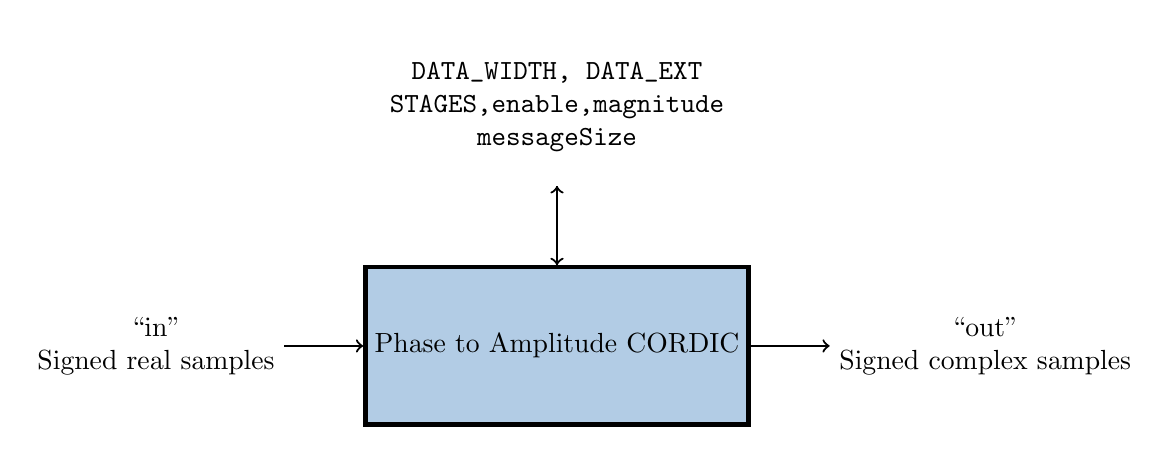
\begin{tikzpicture}[% List of styles applied to all, to override specify on a case-by-case
			every node/.style={
				align=center,  		% use this so that the "\\" for line break works
				minimum size=2cm	% creates space above and below text in rectangle
			},
			every edge/.style={draw,thick}
		]
		\node[rectangle,ultra thick,draw=black,fill=blue](R2){\Comp};
		\node[rectangle,draw=white,fill=white](R3)[left= of R2]{``in'' \\ Signed real samples};
		\node[rectangle,draw=white,fill=white](R4)[right= of R2]{``out'' \\ Signed complex samples};
		\node[rectangle,draw=white,fill=white](R5)[above= of R2]{\verb+DATA_WIDTH, DATA_EXT+\\ \verb+STAGES,enable,magnitude+\\ \verb+messageSize+};
		\path[->]
		(R3)edge []	node [] {} (R2)
		(R2)edge []	node [] {} (R4)
		(R2)edge []	node [] {} (R5)
		(R5)edge []	node [] {} (R2)
		;
	\end{tikzpicture}
	\captionof{figure}{Top Level Block Diagram}
\end{center}

\newpage

\section*{Source Dependencies}
\subsection*{\comp.hdl}
\begin{itemize}
	\item projects/assets/components/dsp\_comps/phase\_to\_amp\_cordic.hdl/phase\_to\_amp\_cordic.vhd
	\item projects/assets/hdl/primitives/dsp\_prims/dsp\_prims\_pkg.vhd
	      \subitem projects/assets/hdl/primitives/dsp\_prims/cordic/src/cordic\_pr.vhd
	      \subitem projects/assets/hdl/primitives/dsp\_prims/cordic/src/cordic.vhd
	      \subitem projects/assets/hdl/primitives/dsp\_prims/cordic/src/cordic\_stage.vhd
	\item projects/assets/hdl/primitives/misc\_prims/misc\_prims\_pkg.vhd
	      \subitem projects/assets/hdl/primitives/misc\_prims/round\_conv/src/round\_conv.vhd
	      	\item projects/assets/hdl/primitives/util\_prims/util\_prims\_pkg.vhd
	      \subitem projects/assets/hdl/primitives/util\_prims/pd/src/peakDetect.vhd
\end{itemize}

\begin{landscape}
\section*{Component Spec Properties}
\begin{scriptsize}
	\begin{tabular}{|p{3cm}|p{1.5cm}|c|c|c|c|c|p{7cm}|}
		\hline
		\rowcolor{blue}
		Name               & Type   & SequenceLength & ArrayDimensions & Accessibility      & Valid Range & Default & Usage                                                               \\
		\hline
		\verb+DATA_WIDTH+  & UChar  & -              & -               &          & -           & -       & Input (real) and Output (I/Q) data width                            \\
		\hline
		\verb+DATA_EXT+    & UChar  & -              & -               &          & -           & -       & CORDIC requirement: \# of extension bits                            \\
		\hline
		\verb+STAGES+      & UChar  & -              & -               &          & -           & -       & Number of CORDIC stages implemented                                 \\
		\hline
		\verb+messageSize+ & UShort & -              & -               & Writable & -           & 8192    & Number of bytes in output message (Not implemented by Version 2) \\
		\hline
		\verb+enable+      & Bool   & -              & -               & Writable & -           & True    & Enable(true) or bypass(false)                                       \\
		\hline
		\verb+magnitude+   & UShort & -              & -               & Writable & -           & 16384   & Magnitude of output \scriptsize\begin{verbatim} * +2^(DATA_WIDTH)-1
			to -2^(DATA_WIDTH)\end{verbatim}\\
		\hline
	\end{tabular}
\end{scriptsize}

\section*{Worker Properties}
\subsection*{\comp.hdl}
\begin{scriptsize}
	\begin{tabular}{|p{3cm}|p{2cm}|c|c|c|c|c|p{1cm}|p{6cm}|}
		\hline
		\rowcolor{blue}
		Type         & Name              & Type & SequenceLength & ArrayDimensions & Accessibility & Valid Range & Default & Usage                                    \\
		\hline
		SpecProperty & \verb+DATA_WIDTH+ & -    & -              & -               & Parameter     & 8-16        & 16      & Input (real) and Output (I/Q) data width \\
		\hline
		SpecProperty & \verb+DATA_EXT+   & -    & -              & -               & Parameter     & 6           & 6       & CORDIC requirement: Number of extension bits \\
		\hline
		SpecProperty & \verb+STAGES+     & -    & -              & -               & Parameter     & 8-16        & 12      & Number of CORDIC stages implemented      \\
		\hline
		Property & \verb+PEAK_MONITOR+     & Bool    & -              & -               & Parameter     & Standard        & true      & Enable/Disable build-time inclusion of peak monitor circuit\\
		\hline
		Property & \verb+peak+     & Short & -              & -               & Volatile & Standard        & 0 & Peak value of I/Q output (valid when PEAK\_MONITOR=true)\\
		\hline
	\end{tabular}
\end{scriptsize}
\subsection*{\comp.rcc}
\begin{scriptsize}
	\begin{tabular}{|p{3cm}|p{2cm}|c|c|c|c|c|p{1cm}|p{6cm}|}
		\hline
		\rowcolor{blue}
		Type         & Name              & Type & SequenceLength & ArrayDimensions & Accessibility & Valid Range & Default & Usage                                    \\
		\hline
		SpecProperty & \verb+DATA_WIDTH+ & -    & -              & -               & Parameter     & 8-16        & 16      & Input (real) and Output (I/Q) data width \\
		\hline
		SpecProperty & \verb+DATA_EXT+   & -    & -              & -               & Parameter     & 6           & 6       & CORDIC requirement: Number of extension bits \\
		\hline
		SpecProperty & \verb+STAGES+     & -    & -              & -               & Parameter     & 8-16        & 12      & Number of CORDIC stages implemented      \\
		\hline
		Property & \verb+PEAK_MONITOR+     & Bool    & -              & -               & Parameter     & Standard        & true      & Enable/Disable build-time inclusion of peak monitor circuit\\
		\hline
		Property & \verb+peak+     & Short & -              & -               & Volatile & Standard        & 0 & Peak value of I/Q output (valid when PEAK\_MONITOR=true)\\
		\hline
		Property & \verb+AdditionalDelay+     & UChar & -              & -               & Parameter        & Standard & 2 & Additional number of delays over CORDIC stages (STAGES) to match HDL implementation.\\
		\hline
		Property & \verb+StageDelay+     & UChar & -              & -               & Parameter        & 0-255 & STAGES + AdditionalDelay & Number of delays to match HDL implementation.\\
		\hline
	\end{tabular}
\end{scriptsize}

\section*{Component Ports}
\begin{scriptsize}
	\begin{tabular}{|M{2cm}|M{1.5cm}|M{4cm}|c|c|M{9cm}|}
		\hline
		\rowcolor{blue}
		Name & Producer & Protocol           & Optional & Advanced & Usage                  \\
		\hline
		in   & false    & rstream\_protocol  & false    & -        & Signed real samples    \\
		\hline
		out  & true     & iqstream\_protocol & false    & -        & Signed complex samples \\
		\hline
	\end{tabular}
\end{scriptsize}

\section*{Worker Interfaces}
\subsection*{\comp.hdl}
\begin{scriptsize}
	\begin{tabular}{|M{2cm}|M{1.5cm}|M{4cm}|c|M{10cm}|}
		\hline
		\rowcolor{blue}
		Type            & Name & DataWidth & Advanced                & Usage                  \\
		\hline
		StreamInterface & in   & 16        & & Signed real samples    \\
		\hline
		StreamInterface & out  & 32        & InsertEOM=1 & Signed complex samples \\
		\hline
	\end{tabular}
\end{scriptsize}
\end{landscape}

\section*{Control Timing and Signals}
The Phase to Amplitude CORDIC worker uses the clock from the Control Plane and standard Control Plane signals. This worker has a start-up transient delay of \verb+STAGES++2 valid samples. This means that once the input is ready and valid and the output is ready, it takes that many valid input samples before the first output sample is made available. The delays for this worker are itemized be as follows:
\begin{itemize}
	\item 0 : pr\_cordic.vhd
	\item 1 : pr\_cordic.vhd/cordic\_pr.vhd
	\item STAGES : pr\_cordic.vhd/cordic\_pr.vhd/cordic.vhd/cordic\_stage.vhd 
	\item 1 : cordic\_pr.vhd/round\_conv.vhd
\end{itemize}

\begin{tabular}{|M{4.5cm}|M{1cm}|M{1cm}|M{1.5cm}|M{2cm}|M{1cm}|M{1cm}|M{2.5cm}|}
	\hline
	\rowcolor{blue}
	Latency                      \\
	\hline
	\verb+STAGES++2 clock cycles \\
	\hline
\end{tabular}

\begin{landscape}
\section*{Worker Configuration Parameters}
\subsubsection*{\comp.hdl}
%\input{../../\ecomp.hdl/configurations.inc}
\section*{Performance and Resource Utilization}
\subsection*{\comp.hdl}
%\input{../../\ecomp.hdl/utilization.inc}
\end{landscape}
\newpage

\section*{Test and Verification}
This component is tested via the unit test automation feature of the framework.  The component's .test/ contains XML files that describe the combinations of tests.\medskip

Two test cases are employed to verify the Phase to Amplitude CORDIC component:

\begin{enumerate}
	\item Disabled. The real input data is passed through the worker and made available on lower 16 bits of the complex output.
	\item Constant output frequency: A python script creates a file containing a constant value. The CORDIC produces a complex output frequency according to the equation \ref{eq:output_freq}.
\end{enumerate}

The plots below show the input (real) and output data (Q-leg showing all samples, I-leg zoomed into one cycle) for testing a Phase to Amplitude CORDIC having the default parameter set. The input file shows a DC value of 2048, and 16384 real samples.  The output file shows the converted complex waveform having $DC value/2^{DATA\_WIDTH}$=2048/$2^{16}$=0.03125 Hz, and 16384 complex samples.

\begin{figure}[ht]
	\centering
	\begin{minipage}{.5\textwidth}
		\centering\includegraphics[width=1.0\linewidth]{input}
		\captionof{figure}{Time Domain}
		\label{fig:input_tdomain}
	\end{minipage}%
	\begin{minipage}{.5\textwidth}
		\centering\includegraphics[width=1.0\linewidth]{input_fft}
		\captionof{figure}{Frequency Domain}
		\label{fig:input_fdomain}
	\end{minipage}
\end{figure}

\begin{figure}[ht]
	\centering
	\begin{minipage}{.5\textwidth}
		\centering\includegraphics[width=1.0\linewidth]{output}
		\captionof{figure}{Time Domain}
		\label{fig:output_tdomain}
	\end{minipage}%
	\begin{minipage}{.5\textwidth}
		\centering\includegraphics[width=1.0\linewidth]{output_fft}
		\captionof{figure}{Frequency Domain}
		\label{fig:output_fdomain}
	\end{minipage}
\end{figure}


\end{document}
